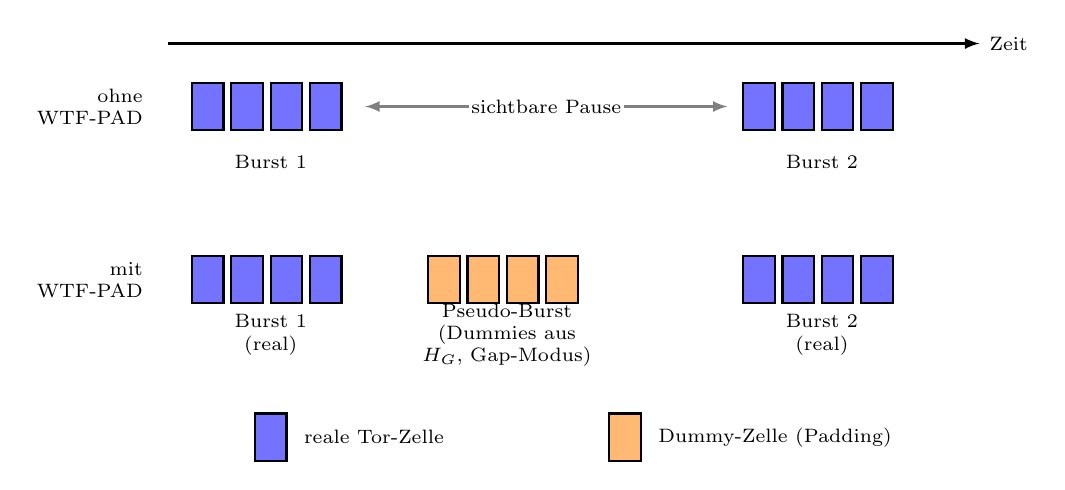
\begin{tikzpicture}[
    >=latex,
    every node/.style={font=\small},
    realcell/.style={
        draw, thick,
        minimum width=4mm, minimum height=6mm,
        inner sep=0pt,
        fill=blue!55
    },
    dummycell/.style={
        draw, thick,
        minimum width=4mm, minimum height=6mm,
        inner sep=0pt,
        fill=orange!55
    },
    rowlbl/.style={font=\scriptsize, anchor=east, align=right},
    grouplbl/.style={font=\scriptsize, align=center}
]

% Zeitachse
\draw[->, thick] (-3mm, 18mm) -- (100mm, 18mm)
    node[right, font=\scriptsize] {Zeit};

% =========================================================
% Obere Zeile: ohne WTF-PAD
% =========================================================
\node[rowlbl] at (-5mm, 10mm) {ohne\\WTF-PAD};

% Burst 1
\foreach \i in {0,1,2,3} {
    \node[realcell] at ({\i*5mm + 2mm}, 10mm) {};
}
\node[grouplbl] at (10mm, 3mm) {Burst 1};

% Burst 2
\foreach \i in {0,1,2,3} {
    \node[realcell] at ({70mm + \i*5mm + 2mm}, 10mm) {};
}
\node[grouplbl] at (80mm, 3mm) {Burst 2};

% Pause-Markierung
\draw[<->, gray, thick] (22mm, 10mm) -- (68mm, 10mm);
\node[font=\scriptsize, fill=white, inner sep=1pt] at (45mm, 10mm)
    {sichtbare Pause};

% =========================================================
% Untere Zeile: mit WTF-PAD
% =========================================================
\node[rowlbl] at (-5mm, -12mm) {mit\\WTF-PAD};

% Burst 1 (real)
\foreach \i in {0,1,2,3} {
    \node[realcell] at ({\i*5mm + 2mm}, -12mm) {};
}
\node[grouplbl] at (10mm, -19mm) {Burst 1\\\scriptsize (real)};

% Pseudo-Burst (Dummies, Gap-Modus)
\foreach \i in {0,1,2,3} {
    \node[dummycell] at ({30mm + \i*5mm + 2mm}, -12mm) {};
}
\node[grouplbl, text width=34mm] at (40mm, -19mm)
    {Pseudo-Burst\\\scriptsize (Dummies aus $H_G$, Gap-Modus)};

% Burst 2 (real)
\foreach \i in {0,1,2,3} {
    \node[realcell] at ({70mm + \i*5mm + 2mm}, -12mm) {};
}
\node[grouplbl] at (80mm, -19mm) {Burst 2\\\scriptsize (real)};

% =========================================================
% Legende
% =========================================================
\node[realcell] at (10mm, -32mm) {};
\node[font=\scriptsize, anchor=west] at (13mm, -32mm) {reale Tor-Zelle};

\node[dummycell] at (55mm, -32mm) {};
\node[font=\scriptsize, anchor=west] at (58mm, -32mm) {Dummy-Zelle (Padding)};

\end{tikzpicture}
